\chapter{Biological Neural Networks} 
\label{chapter-biological} 

In this chapter, we describe our experiments to test and extend the findings in \cite{dyballa_manifold_2021} on a different  data set collected from the retina.

\section{Neural tensor for retina}
The neural spiking data \cite{dyballa_manifold_2021} were collected from lab experiments with the setup shown in the figure below. Six different types of flow stimuli developed in \cite{visual-flow} were flashed in front of the mouse. The electrodes recorded the neural output from the mouse's retina while it viewed each flow stimuli moving in eight directions respectively. The neural recordings were encoded in peristimulus (PSTH) diagrams, each of which showed the firing rate of one neuron over time for the eight directions respectively. In the PSTH diagram the brighter pixels indicate higher firing rates.
\begin{figure}[H]
    \centering
        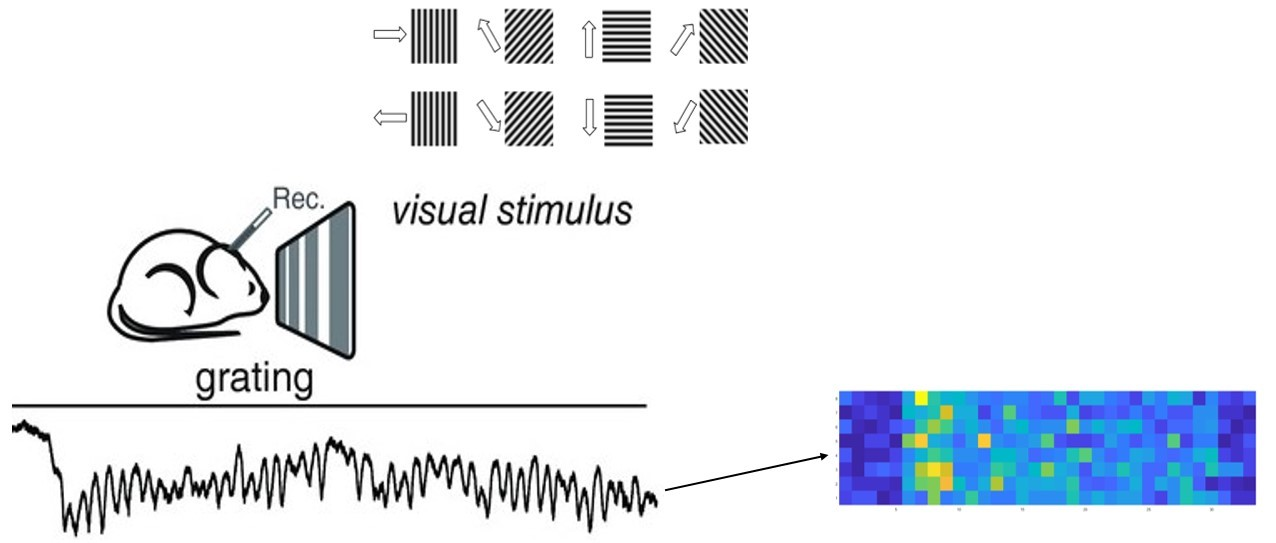
\includegraphics[width=0.6\textwidth]{figures/biological/biological-input-output.jpg}
        \caption{Visualising neural data from lab experiments.}
\end{figure}

\par The neural spiking data is of three dimensions: the first dimension represents the $698$ neurons; the second dimension represents the six different types of stimuli; the third dimension represents the vectorized PSTH diagrams, each of which has $8\times 33 = 264$ pixels. This gives us a $3$-way tensor:

\begin{defn}[Neural tensors]
    Suppose $\mathcal{S}$ is a set of flow stimuli $\mathcal{S} = \{s_1, s_2,\dots, s_K\}$, each moving over  $T$ time steps. The \underline{neural population response} of a set of $N$ neurons to some stimulus $s_i$ over time is $\mathcal{N} = \{\vec{n}_1, \vec{n}_2, \dots, \vec{n}_N\},$ where $\vec{n}_i \in \mathbb{R}^{T}$. 

    Each \underline{neural tensor} encodes the neural population response of $N$ neurons to $K$ flow stimuli over $T$ time steps and is thus a $3$-way $N$-by-$K$-by-$T$ tensor.
\end{defn}

\section{Neural factors for retina}
We implement the Non-negative Tensor Factorization (NTF) using the Tensor Toolbox for MATLAB \cite{tensortoolbox}. Our algorithm is as follows:

\setcounter{algocf}{1}
\begin{algorithm}[H]
\setstretch{1}
\caption{Algorithm for NTF on retina tensor.}\label{alg:factors-retina}
\KwData{Neural tensor for retina.}
\KwResult{$R$ tensor factors for retina.}
\DontPrintSemicolon
import data as X, X = tensor(X) \;
chosen rank, R = 35 \;
n\_repetitions = 10, initialize errors with zeros \; 
\For{r from 1 to R}{
\For{rep from 1 to n\_repetitions}{
NTF: M = cp\_opt(X, r, 'init', 'rand' , 'lower', 0) \;
error = norm(X - tensor(M)) / norm(X); \;
add error to the array of errors \;
}
}
F\_neuron = M.u\{1\}, F\_stimuli = M.u\{2\}, F\_time = M.u\{3\} \;
save the factors \;
\end{algorithm}

We plot the reconstruction error curves to compare the performance of tensor CP decomposition when different optimization methods are used. ALS with random initialization and regular direct optimization perform better than non-negative direct optimization. However, since the neural output from biological neural networks is always non-negative, in order to ensure the interpretability of the resulting tensor factors in the context of our application, we choose to use non-negative direct optimization despite its relatively worse performance (which is not a crucial concern in our application since the neural factors obtained in this process are still good enough approximation of the original neural data).

\begin{figure}[H]
\centering
    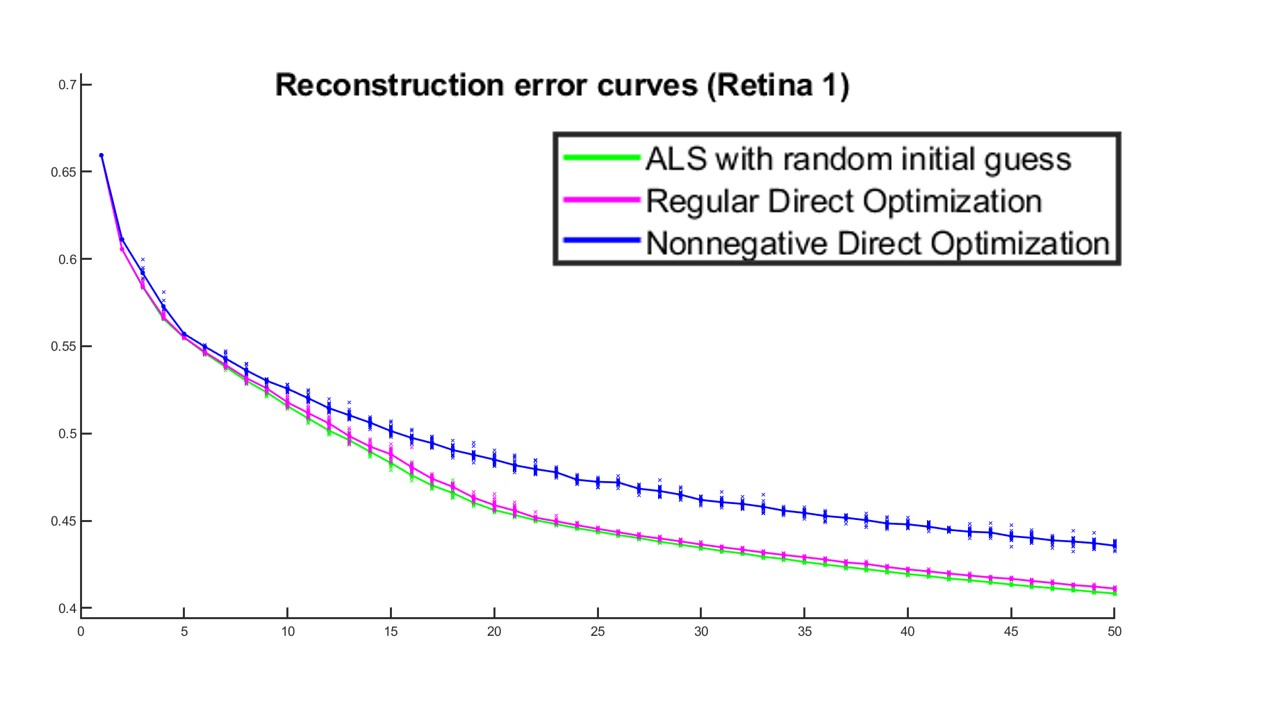
\includegraphics[width=0.6\textwidth]{figures/biological/retina1-reconstruction-error.jpg}
     \caption{Reconstruction errors of different optimization methods.}
\end{figure}  

We can visualize the resulting tensor factors:
\begin{figure}[H]
    \centering
        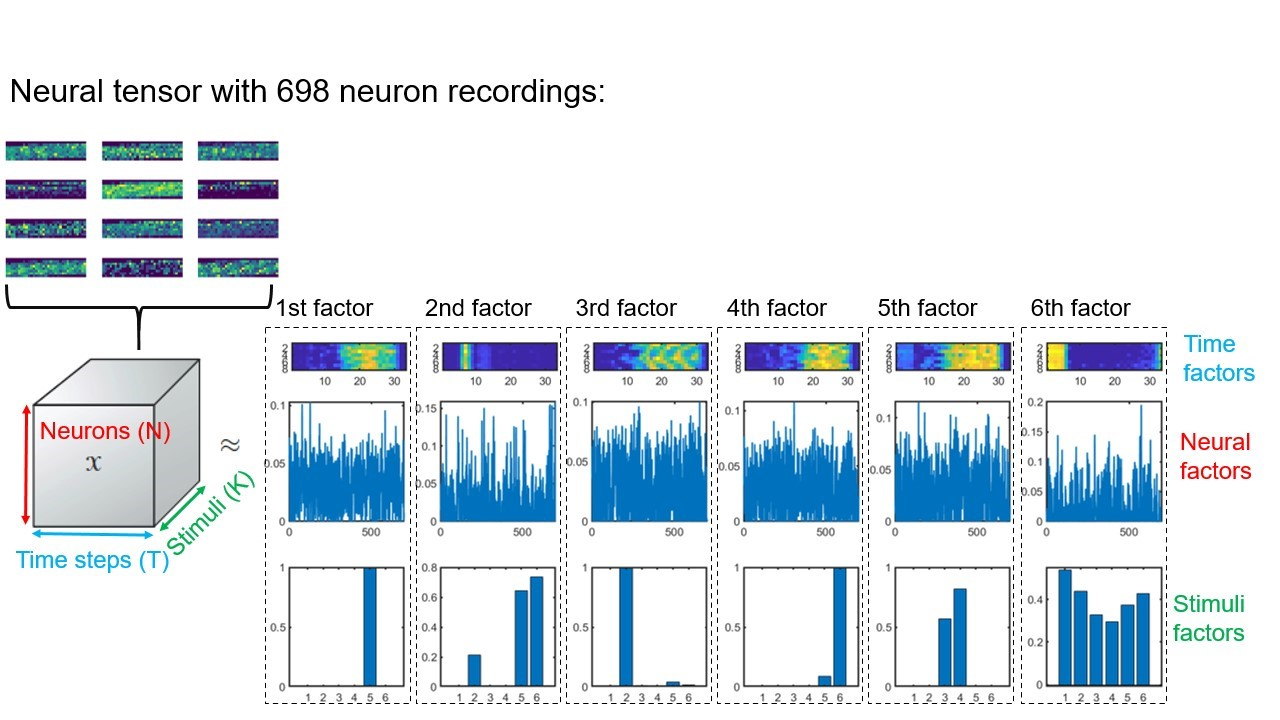
\includegraphics[width=0.8\textwidth]{figures/biological/retina-factors.jpg}
        \caption{First six tensor factors for retina.}
    \end{figure} 

\section{Neural manifold for retina}
The tensor factors form what we call the ``neural matrix" of dimension $(N,R)$, where $N$ is the number of neurons and $R$ is the chosen rank. Since the tensor factors provide an approximation of the original neural spiking data, we use PCA to project neural matrix onto a linear subspace with the same dimension, i.e., the number of components is $R$. We then use k-means clustering to label the clusters by distances in the lower-dimensional linear subspace. By choosing the optimal number of clusters to be six based on the experiments, we obtain the neural manifold for retina. In the following plot, each point represents a neuron. From the visualization below, the neural manifold for retina is discontinuous and the PSTH diagrams within each cluster are similar. This implies that neurons form disconnected clusters grouped by their firing patterns, implying that neurons have distinct stimuli preferences. By using the the connections between neural manifolds and neural circuits explained in \label{networks-manifolds}, we can already infer that the neural networks in retina are characterized by isolated neural circuits. We extend this result further by quantifying the degree of continuity in the next section.
  \begin{figure}[H]
        \centering
             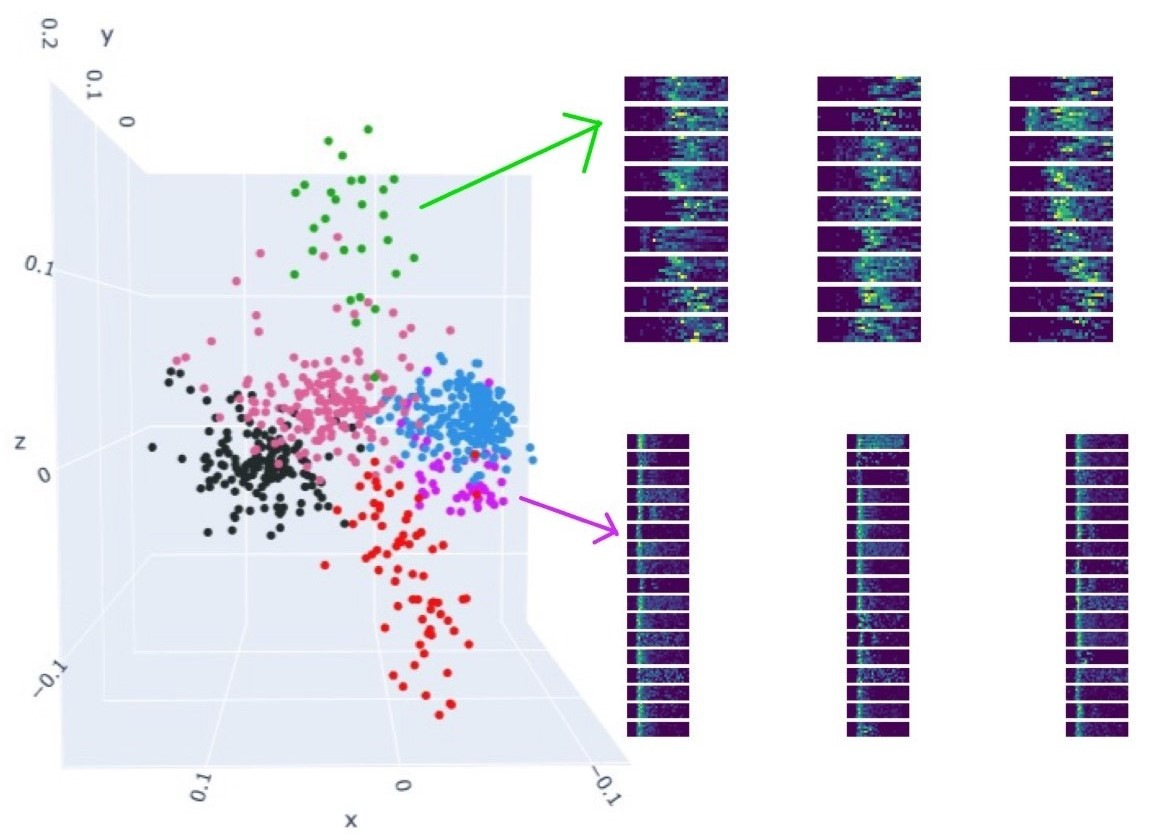
\includegraphics[width=0.7\textwidth]{figures/biological/retina-manifold-with-psth.jpg}
            \caption{Neural manifold for retina is discontinuous.}
        \end{figure} 

\subsection{Quantifying the continuity of the manifold}
Following the method proposed in \cite{dyballa_manifold_2021}, we compute the mean flow ratio (MFR) as a quantifiable measure to compare the continuity of the respective neural manifolds: the smaller the MFR, the more discontinuous the neural manifold is, and vice versa. The algorithm is outlined on the next page. The MFR of the retina neural manifold computed from our algorithm is $\phi_G = 0.56$. Now we compare the results with V1 using results from \cite{dyballa_manifold_2021}: the neural manifold for V1 is continuous in the visualizatoin below and the MFR of V1 is $\phi_G = 0.91$ as concluded in . The difference in the MFRs suggests that the neural manifold for V1 is much more continuous than retina. Thus, we can conclude that the neural circuit in V1 has much higher connectivity than retina. The results in this chapter will be used again in the next chapter to compare with results from the artificial neural networks.
 \begin{figure}[H]
        \centering
             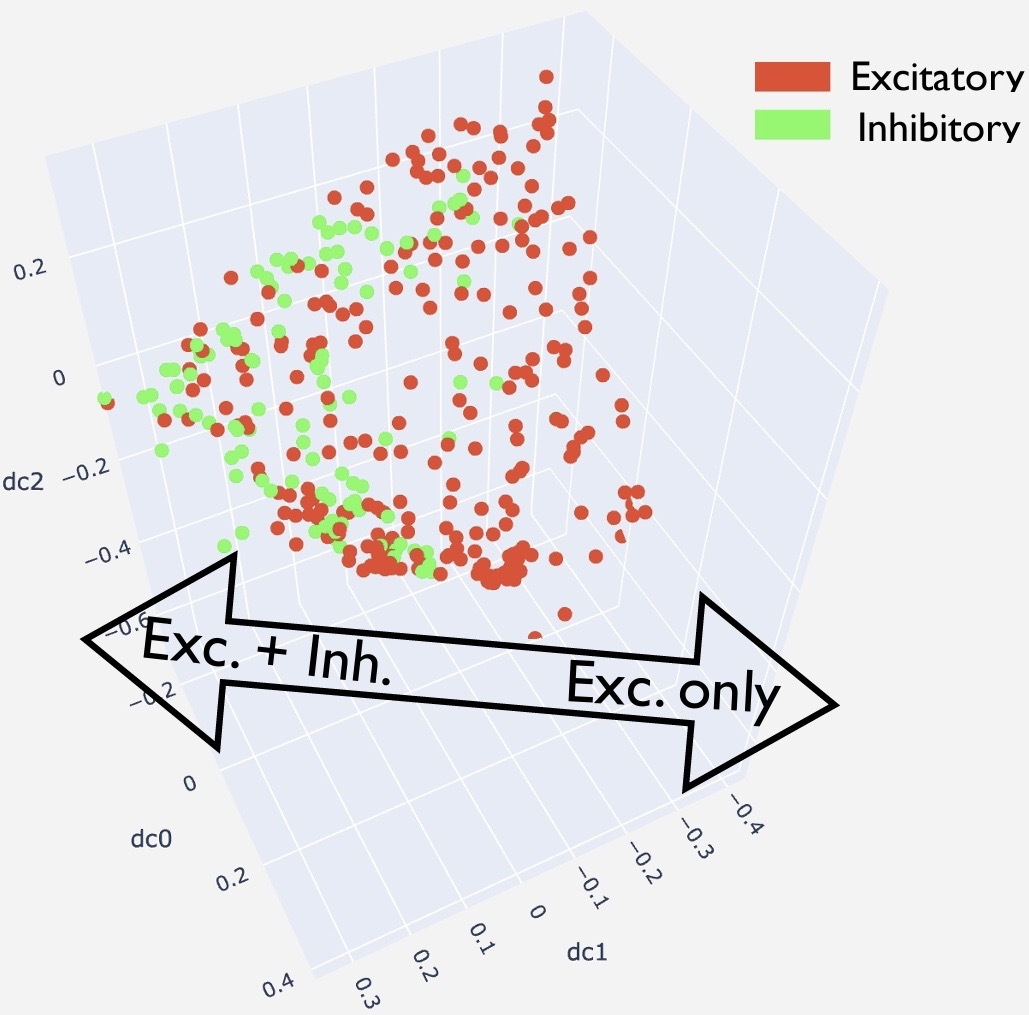
\includegraphics[width=0.45\textwidth]{figures/biological/v1-manifold.jpg}
            \caption{Neural manifold for V1 is continuous. The neurons are colored by excitatory and inhibitory functions and the two clusters overlap each other.}
        \end{figure} 
% The mean flow ratio has its origin in the maximum flow problem, a classic problem in graph theory originally formulated as a means to optimize railway traffic between cities \cite{schrijver_history_2002}.

\setcounter{algocf}{2}
\begin{algorithm}[H]
\setstretch{1}
\caption{Algorithm for computing the mean flow ratio.}\label{alg:mean-flow-ratio}
\DontPrintSemicolon
\KwData{points on the neural manifold, $\xx_1, \dots, \xx_N \in \mathcal{M}$.}
\KwResult{mean flow ratio for the neural manifold, $\phi_G$.}
kernel bandwidth, $\epsilon \coloneqq \frac{1}{N}\sum_{i=1}^N \min_{j: \xx_j \neq \xx_i}\|\xx_i - \xx_j\|^2$\;
Gaussian kernel\footnote{In fact, we can choose any symmetric, positive semi-definite similarity kernel. But Gaussian kernel gives a physically intuitive construction as it effectively considers a ball of radius $\epsilon$ around each data point.}, $k(\xx_i, \xx_j) = \exp(-\|\xx_i - \xx_j\|^2/\epsilon)$ \;
weight matrix $W, W_{i, j}\coloneqq {k_\epsilon}(\xx_i, \xx_j)$\;
degree of node $\xx_i$, $d(\xx_i) \coloneqq \sum_{j=1}^N W_{i,j}$\;
anisotropic Gaussian kernel, $\Tilde{k_\epsilon}(\xx_i, \xx_j) \coloneqq \frac{k_\epsilon(\xx_i, \xx_j)}{d(\xx_i)d(\xx_j)}$ \;
anisotropic weight matrix,$\Tilde{W}, \Tilde{W}_{i, j}\coloneqq \Tilde{k_\epsilon}(\xx_i, \xx_j)$\;
build graph $G = (V, E)$, weight of the edge ($\xx_i$, $\xx_j$) is $\Tilde{W}_{i, j}$ \;
edge resistance, $R_{i, j} = 1/\Tilde{W}_{i, j}$ \;
compute effective resistance $R^{\text{eff}}_{i, j}$, using \cite{effective-resistance}\;
effective conductance, $C^{\text{eff}}_{i, j} = 1/R^{\text{eff}}_{i, j}$\;
build graph $G_C$, weight of the edge ($\xx_i$, $\xx_j$) is $C^{\text{eff}}_{i, j}$  \;
\For{i from 1 to N}{
\For{j from 1 to N, $j\neq i$}{
SumAll += \text{maxflow}(i, j)\;
}
\For{k: k is a neighbor of i}{
SumNeighbors += \text{maxflow}(i, k)
}
flow ratio of node $\xx_i$, $\rho_i$ = SumAll/SumNeighbors\;
}
mean flow ratio of graph $G$, $\phi_G = \sum_{i=1}^N \rho_i.$
\end{algorithm}
